\chapter{Diversidad de Rango}

Los primeros análisis se enfocaron en buscar hechos relevantes que propiciaron las migraciones de palabras,  siendo oportuna la información histórica.  El capítulo anterior busco ver a cada idioma como un conjunto “universal” donde las propiedades que lo caracterizan  son comunes en cada uno y siguen siendo válidas a pesar de reducir los elementos que los componen al extraer palabras. 

En esta sección se buscará entender cómo son las variaciones de palabras a  lo largo del tiempo, para ello  se enfocara el estudio a cuantificar que tan diferentes son las listas de los préstamos de un idioma en otro,  ya que estas listas están ordenadas por rango, (donde el rango más bajo es la palabra más común en ese año y la de rango más alto la menos utilizada)  una misma palabra puede ocupar distintos cargos en diferentes años,  o  para un mismo rango existe una diversidad de palabras que lo ocupan, esta idea es más adecuada ya hay palabras que no  aparecen en todos los años del análisis,  sin embargo en todos las listas  hay palabras hasta cierta posición (rango).   

La propuesta de la diversidad de rango ha sido utilizada en corpus donde se clasifican las palabras más comunes de seis diferentes idiomas \cite{tesis.sergio} y en deportes y juegos con diferentes criterios para establecer un orden \cite{tesis.jama}. En cada caso,  el algoritmo para llegar a la diversidad se describe de la siguiente manera:


\begin{enumerate}
	
	\item Se fijan un año inicial $t_{o}$ y uno final $t_{o}$, construyendo un intervalo de años a evaluar $\Delta\,t = t_{f}- t_{o}$.
	
	\item Se toma el primer rango de todos los años en el intervalo y se cuenta el número de palabras que son distintas en ese rango. Esta cantidad será la diversidad para el rango uno.
	
	\item Se prosigue con el segundo rango y se vuelve a contar cuántas palabras son diferentes en todo el periodo de tiempo.  Con ello se obtiene la diversidad para el rango dos. 
	
	\item Ya que las listas de préstamos de un idioma en otro no son homogéneas en cantidad, el procedimiento anterior se repetirá hasta el rango mínimo que poseen todas las listas,  así se asegura tener una homogeneidad en el tamaño.
	
	\item Se normalizan  los valores dividiendo cada resultado entre el número de años comprendidos del intervalo $\Delta\,t$, obteniendo  la diversidad de rango $d(k)$.
	
	
\end{enumerate}


Antes de mostrar los resultados, se espera  que los valores de $d(k)$ sean cercanos a cero cuando  para un rango $k$, las cantidad de palabras que ocupan ese rango sea menor. En caso de que la diversidad sea cercana a uno,  significa que hay una mayor cantidad de palabras que ocupan el rango $k$. 


Tras graficar el rango contra la diversidad, se observó que en todas las combinaciones (a pesar de que algunas tuvieran más datos)  la tendencia de la diversidad  se asemeja a una función de distribución cumulativa logarítmica  normal, la cual depende del rango $k$, y la desviación estándar $\sigma$.

\begin{equation}
	\label{ec.cumulativa}
	F(k) = \Phi \left ( \frac{ln(k)}{\sigma} \right )\,\,\,\,k\geq 0; \sigma \geq 0
\end{equation}

Donde $\Phi$ es la función cumulativa de la distribución normal, que ademas del rango y la desviación estándar, depende del promedio $\mu$.

\begin{equation}
	\label{ec.distribucionnormal}
	\Phi(t) = \frac{1}{\sigma\sqrt{2\pi}} \int_{-\infty}^{t}  e^{ \frac{ - \left ( x-\mu \right )^{2}}{2\sigma^2}  } dx	
\end{equation}



\section{Ajuste de Datos}


Se intentaron ajustar los puntos de la diversidad con esta distribución, sin embargo al ser pocos los rangos (la mayor cantidad de rangos en cualquier combinación fue de 290),  la curva descrita  no ajusta correctamente;  si se tuvieran mayor cantidad de rangos del orden de $10^{3}$ o $10^{4}$ el ajuste es más preciso.  Para solucionar este problema se propuso hacer un ajuste lineal con la función logarítmica  de la siguiente forma:


\begin{enumerate}
	\item Se propone una función para la diversidad $d(k)$ de la forma
	
	\begin{equation}
	\label{ec.ajuste}
	y(k) =  \alpha \, ln(k) + \beta
	\end{equation}
	
	\item Al realizar los cambios de variable $\hat{Y} = y(k)$ y $X = ln(k)$, se obtiene una ecuación lineal para $k$.
	$$ \hat{Y} =  \alpha X + \beta$$
	
	\item Para encontrar los parámetros $\alpha$ y $\beta$, se utilizó el método de mínimos cuadrados, minimizando la suma de los cuadrados de los errores.  
	
	\item Conocidos los valores de $X$, la diversidad $Y$ y la cantidad de valores $n$,  se calcularon los valores muestrales de las medias ($\mu_{X}$ y $\mu_{Y}$), las varianzas ($\sigma^{2}_{X}$ $\sigma^{2}_{Y}$)  y la covarianza de las dos variables  $\sigma_{XY}$.
	
	$$ \bar{X} = \frac{1}{n} \sum_{i=1}^{n} X_{i} $$
	
	$$ \bar{Y} = \frac{1}{n} \sum_{i=1}^{n} Y_{i} $$
	
	$$ \sigma^{2}_{X} = \frac{1}{n} \sum_{i=1}^{n} \left (X_{i} -\bar{X}\right )^{2} $$
	
	$$ \sigma^{2}_{Y} = \frac{1}{n} \sum_{i=1}^{n} \left (Y_{i} -\bar{Y}\right )^{2} $$
	
	$$ \sigma_{XY} = \frac{1}{n} \sum_{i=1}^{n} \left (X_{i} - \bar{X}\right )  \left (Y_{i} - \bar{Y} \right ) $$
	
	\item Así los parámetros se expresan como
	
	$$ \alpha = \frac{\sigma_{XY}}{\sigma^{2}_{X}} $$
	
	$$ \beta = \bar{Y} - \alpha \bar{X}$$
	
	\item Calculados cada punto del ajuste (\ref{ec.ajuste}) $y_{i}$ y los valores calculados de diversidad $f_{i}$, para comprobar que tan adecuado es el ajuste se obtiene el coeficiente de determinación $R^{2}$.
	
	\begin{equation}
	\label{ec.rcuadrado}
	R^{2} = \frac{\sigma_{XY}}{\sigma^{2}_{X} \sigma^{2}_{Y}} \,\, = \,\, 1- \frac{\sum_{i=1}^{n} \left( y_{i} - f_{i}\right)^{2} }{\sum_{i=1}^{n} \left (y_{i} -\bar{Y}\right )^{2}}
	\end{equation}
	
	
	 
\end{enumerate}


Valores de $R^{2}$ próximos a 1 indicarán que existe una relación lineal ( en este caso logarítmica por el cambio de variable) exacta entre las dos variables.

Para tener una única ecuación para la diversidad de rango de todas las posibles  combinaciones, se establecieron a $\alpha = 0.17\pm 0.04$ y $\beta = -0.18 \pm 0.08$, obtenidas a partir del promedio de cada $\alpha$ y $\beta$ de los ajustes individuales, quedando la diversidad de rango como:

\begin{equation}
	\label{ec.gen_ajs}
	d(k) = 0.17\,ln(k) - 0.18
\end{equation} 




\clearpage

\begin{figure}[h!]
	\centering
	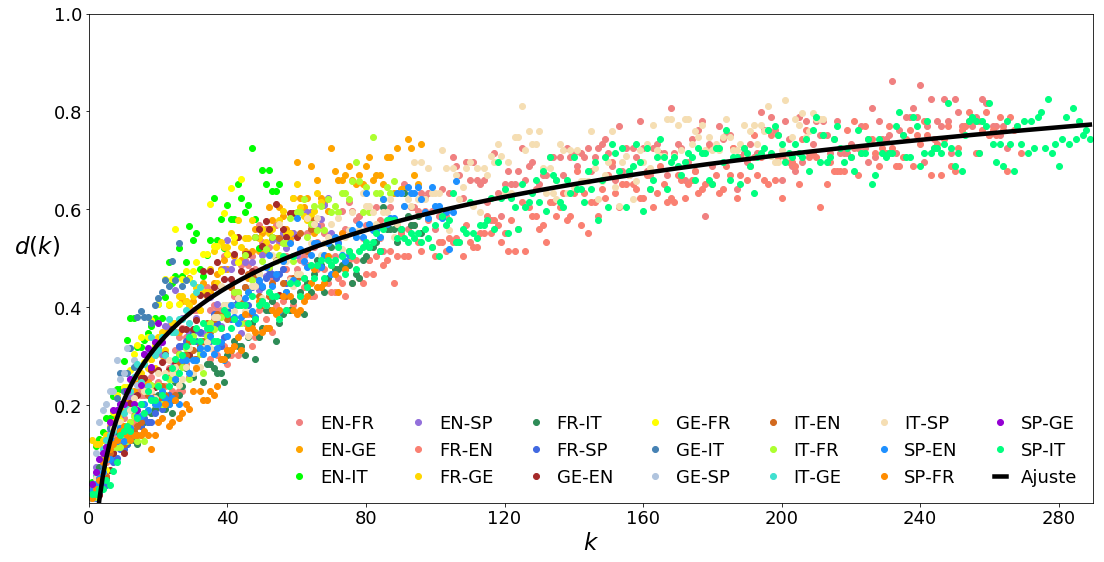
\includegraphics[scale=.39]{Cap_6/DR_gen.png}
	\label{fig.DR_gen}
	\caption{Diversidad de rango entre idiomas.}
\end{figure}
 

La figura anterior muestra la diversidad de cada pareja de idiomas junto con la ecuación anterior; a pesar de que no todas las combinaciones tienen la misma cantidad de rangos en sus listas año a año, cada distribución de puntos asemeja siempre a una curva logarítmica cuya mayor diversidad se encuentra conforme el rango $k$ se acerca a sus valores más altos.

Como se comentó anteriormente cada pareja de idiomas presentó diferentes valores de $\alpha$ y $\beta$ tras ajustar la diversidad y asi obtener una ecuación de ajuste; la siguiente tabla muestra los parámetros anteriores, así como los valores de $\mu$, $\sigma$, $R^{2}$ y $k_{min}$ que es el rango minimo que tienen todas las listas para la pareja de idiomas y donde se implementó el algoritmo de diversidad.

\begin{table}[h!]
	\centering
	\begin{tabular}{ccccccc}
		\textbf{}                & \textbf{$\mu$} & \textbf{$\sigma$} & \textbf{$k_{min}$} & \textbf{$\alpha$} & \textbf{$\beta$} & \textbf{$R^{2}$} \\
		\textbf{inglés-francés}  & 0.61           & 0.18                & 265                   & 0.18           & -0.23         & 0.94        \\
		\textbf{inglés-alemán}   & 0.49           & 0.19                & 96                    & 0.19           & -0.23         & 0.92        \\
		\textbf{ingles-italiano} & 0.45           & 0.17                & 55                    & 0.17           & -0.10         & 0.91        \\
		\textbf{ingles-español}  & 0.38           & 0.15                & 70                    & 0.15           & -0.14         & 0.88        \\
		\textbf{francés-inglés}  & 0.55           & 0.18                & 269                   & 0.18           & -0.29         & 0.93        \\
		\textbf{francés-alemán}   & 0.42           & 0.16                & 67                    & 0.17           & -0.12         & 0.87        \\
		\textbf{francés-italiano} & 0.35           & 0.16                & 96                    & 0.15           & -0.21         & 0.83        \\
		\textbf{francés-español}  & 0.28           & 0.14                & 57                    & 0.15           & -0.19         & 0.86        \\
		\textbf{alemán-inglés}  & 0.35             & 0.17                & 60                    & 0.18           & -0.22         & 0.88        \\
		\textbf{alemán-francés}   & 0.37           & 0.17                & 44                    & 0.19           & -0.16         & 0.89        \\
		\textbf{alemán-italiano} & 0.31            & 0.15                & 28                    & 0.17           & -0.11         & 0.91        \\
		\textbf{alemán-español}  & 0.22            & 0.08                & 14                    & 0.10           & -0.04         & 0.89        \\
		\textbf{italiano-inglés} & 0.31          & 0.15                & 66                   & 0.15           & -0.18        & 0.86        \\
		\textbf{italiano-francés} & 0.41           & 0.20                & 88                    & 0.20           & -0.28         & 0.85        \\
		\textbf{italiano-alemán}  & 0.26           & 0.12                & 32                    & 0.13           & -0.08         & 0.91        \\
		\textbf{italiano-español}  & 0.22          & 0.19                & 212                    & 0.20           & -0.28         & 0.92       \\
		\textbf{español-inglés}  & 0.41          & 0.18                & 106                   & 0.18           & -0.25        & 0.87        \\
		\textbf{español-francés}   & 0.28           & 0.14                & 75                   & 0.13           & -0.17         & 0.79        \\
		\textbf{español-alemán} & 0.21           & 0.09                & 21                    & 0.11           & -0.02         & 0.86        \\
		\textbf{español-italiano}  & 0.22          & 0.18                & 289                    & 0.18           & -0.28         & 0.95       
	\end{tabular}
	\caption{Parámetros de la diversidad entre idiomas.}
	\label{tab.DR_EN}
\end{table}


\clearpage
\section{La relación entre diversidad de rango y la ley de Zipf}

El proponer una curva logarítmica mostró una similitud aceptable con los puntos de diversidad de rango, sostenido con el valor de $R^{2}$ de cada par de idiomas, a pesar de que el rango mínimo donde se aplicó el método varia entre cada pareja. 

La fiabilidad del ajuste llevó buscar un vínculo entre la ecuación propuesta y  la ley de Zipf [XXX], ya que por un lado la ley de Zipf muestra la relación entre la frecuencia de aparición de las palabras en una determinada lengua con el rango que ocupan en la misma,  mientras que la diversidad cuantifica las distintas palabras que ocupan un mismo rango dentro de una escala temporal.  El término clave en los dos procedimientos es el rango, esta cantidad variable palabra a palabra es el medio por el cual establecer la relación a través de una integral.

Al utilizar la ley de Zipf para rangos bajos (ya que las listas de palabras no contienen más de trescientos elementos):

\begin{equation}
	\label{ec.Zipf_kbajos}
	f(k) = \frac{1}{k^{a}} =  \frac{1}{k}  \,\,\,  \,\,\, \,\,\, con   \,\,\,a=1\ \,\,\,para\,\, k\,\, bajos
\end{equation} 

Si esta ecuación se multiplica por una constante $\alpha$ y se hace una integral indefinida sobre la variable k  entonces:

\begin{equation}
	\label{ec.Zipf_int}
	\int \frac{\alpha}{k}\,\,dk \, = \, \alpha \, ln \left(k\right) + C
\end{equation} 

Si la constante de integración $C = \beta$, entonces se llega a la forma propuesta para la diversidad de rango $d(k)$.  

\begin{subequations}
	\begin{align}
		\label{ec.Zipf_dk}
		\int \alpha f\left(k\right) \,dk \,=\, d(k) \\
		\int \frac{\alpha}{k}\,\,dk \, = \, \alpha \, ln \left(k\right) + \beta	
	\end{align}
\end{subequations}


La relación entre ambas propuestas se pudo haber logrado partiendo de la ecuación de diversidad y con una derivada sobre el rango llegar a la ley de Zipf, sin embargo la razón de hacer la integral sobre la ley de Zipf es que esta ley  ha sido probada con diferentes idiomas e incluso en datos donde los criterios para una clasificación son distintos, en cambio la ecuación logarítmica en la diversidad funciona para conjuntos con $k$ bajos, cuya mayor diversidad se alcanza conforme $k$ se aproxima a sus valores más altos.   El realizar la misma técnica para diferentes conjuntos que cumplan  las premisas anteriores puede afirmar o no la concordancia propuesta, incluso se pueden hacer modificaciones al tomar tomar diferentes versiones para la ley de Zipf o para el ajuste de datos basados en curvas logarítmicas.




